%% Template for MLP Coursework 2 / 6 November 2017 

%% Based on  LaTeX template for ICML 2017 - example_paper.tex at 
%%  https://2017.icml.cc/Conferences/2017/StyleAuthorInstructions

\documentclass{article}
\input{mlp2018_includes}
\usepackage[toc,page]{appendix}

\usepackage[utf8]{inputenc}
 

%% You probably do not need to change anything above this comment

%% REPLACE this with your student number
\def\studentNumber{Ignat Georgiev  |  s1521716}

\begin{document} 


\twocolumn[
\mlptitle{MLP Coursework 1: Learning Algorithms and Regularisation}

\centerline{\studentNumber}

\vskip 7mm
]

\begin{abstract} 
In this paper we investigate the state of the art techniques for deep learning used today. Using our own implementations of the most popular algorithms, we have run several tests on the classical EMINST dataset for an image classification problem and outline the performance, benefits and drawbacks of learning techniques including RMSProp, Adam, Cosine annealing with warm restarts, L2 regularisation and weight decay.
\end{abstract} 

\section{Introduction}
\label{sec:intro}

Deep neural networks have become extremely popular in the recent years. Currently they are the best-performing method for classification problems such as object recognition from images \citep{imagenet} and speech recognition from audio \cite{nn-speech}. This is enabled through training on increasingly large datasets but that is also it's main computational bottleneck: often requiring days of training even for high-performance GPUs.
\\
There have been a significant amount of contributions within the field in the past few years, providing a plethora of options in developing new solutions. However, it is difficult to quantify which solutions work best in general unbiased use cases. In this paper we will explore popular recent advances in classification problems with neural networks and attempt to clarify which solutions provide the best performance, are easy to tune and achieve short training times. 
\\
All experiments will be run on the popular dataset Balanced Extended MNIST \citep{EMNIST} which consists of handwritten digits, lowercase and uppercase letters spanning over 47 different classes. Although not a particularly complex problem, this was chosen due to its availability, popularity and ease to reproduce. The dataset consists of 131,600 examples which are split in test, validation, and train sets of sizes 76\%, 12\% and 12\% respectively.
\\
In this paper we will investigate the 3 most predominant training methods in recent years - Stochastic Gradient Descent (SGD) also referred to as mini-batch gradient descent \citep{SGD_lecture}, RMSProp \citep{RMSProp_lecture} and Adam \citep{Adam}. Afterwards we will explore the effects of variable learning rate schedules, namely cosine annealing and warm restarts of learning which has proposed by \citeauthor{SGDR}. Finally different regularisation techniques will be explored such as the classical L2 regularisation and weight decay as proposed in \citep{loshchilov2018fixing}. Conclusions will be drawn from all of the above with the goal to find the best and most efficient learning methods in neural networks.

\section{Baseline systems}

The goal of this part is to set a baseline for sequential experiments using a simple system with stochastic gradient descent (SGD) and without explicit regularisation. The main aim was to maximise the accuracy of the learning algorithm as well as establishing hyperparameters for fast training. This was approached in 2 stages: first finding a suitable learning rate $\alpha$ and epoch number and then experimenting with various numbers of hidden layers.

\subsection{Learning rate and epoch size}
This section works on the assumption that the learning rate that works best for SGD will also work best for the remaining part of this coursework. This theory will be verified at multiple points into the coursework.
\\
To find an appropriate learning rate and epoch size, a simple neural network was used consisting of
\begin{itemize}
    \itemsep0em 
    \item 1 input, 1 hidden, 1 output layer
    \item ReLu activation units
    \item Cross-Entropy Softmax cost fuction
    \item Stochastic Gradient Descent
    \item Glorot initialisation for weights and Constants initialisation for biases
    \item Batch size of 100
    \item 200 epochs
\end{itemize}

The learning rates tested were \texttt{[1, 0.5, 0.1, 0.05, 0.01, 0.005, 0.001]} based on a pseudo logarithmic scale as suggested in \citep{overviewML}. Results presented in Table \ref{tab:ex1-learn} show that it is  best to have $\alpha = 0.005$ and that accuracy on the validation set starts decreasing after 200 epochs due to overfitting. Other learning rates were not explored due to time limitation.
\begin{table}[tb]
\vskip 3mm
\begin{center}
\begin{small}
\begin{sc}
\begin{tabular}{cccc}
\hline
\abovespace\belowspace
Learn rate & Train acc (\%) & Train error & Training time (s) \\
\hline
\abovespace
1          & 65,70 & 1.3681 & 205 \\
0.5        & 39,68 & 1.4627 & 211 \\
0.1        & 14,00 & 1.4375 & 226 \\
0.05       & 12,85 & 1.0080 & 225 \\
0.01       & 29,48 & 0.5265 & 218 \\
0.005      & 38,84 & 0.5050 & 212 \\
0.001      & 67,92 & 0.7037 & 214 \\
\hline
\end{tabular}
\end{sc}
\end{small}
\caption{Learning performance with varying learning rate.}
\label{tab:ex1-learn}
\end{center}
\vskip -3mm
\end{table}

\subsection{Number of hidden layers}
In this section I have experimented with different numbers of hidden layers ranging from 2 to 5 in an attempt to find the best performing one. For this, the same neural network model was used as in the previous subsection,  $\alpha = 0.005$ but 200 epoch will be run with each neural network to accommodate for the fact that deeper neural networks require more training time.

From \ref{fig:ex1_part2}, it is deduced that the most optimal performance can be obtained from a 3-hidden layer neural network. Interestingly, it approaches it's lowest validation set error near epoch 100, making it faster to train than both 1 and 2 hidden layer models but it is also faster to diverge after epoch 160. It is suspected that the 3 hidden layer model is faster to learn complex functions and thus can achieve good accuracy faster. 4 and 5 hidden layer networks on the other hand are much faster to start diverging which combined with their higher computational cost makes them an unappealing candidate for the remaining part of the coursework.

\begin{figure}[tb]
\vskip 5mm
\begin{center}
\centerline{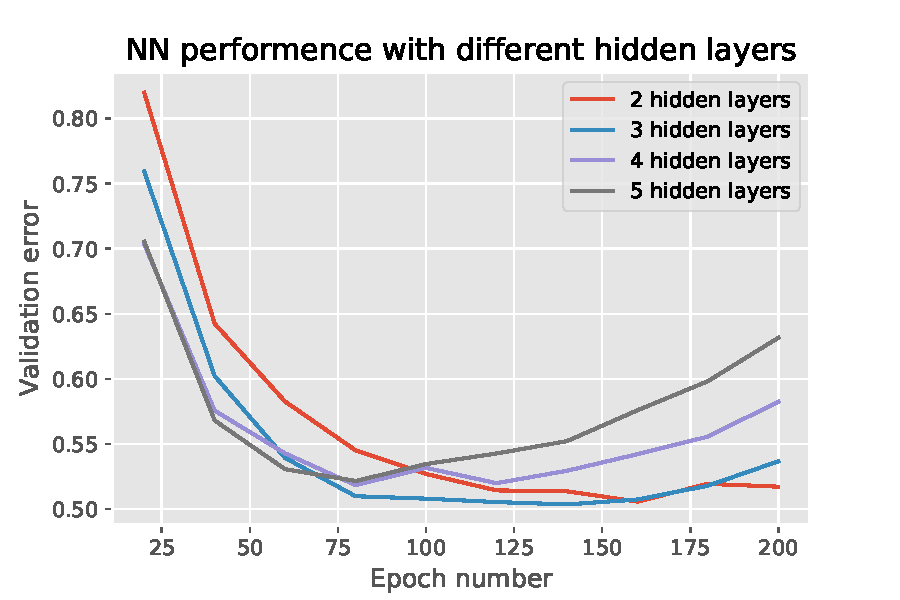
\includegraphics[width=\columnwidth]{ex1_part2.pdf}}
\caption{Validation error over 200 training epochs}
\label{fig:ex1_part2}
\end{center}
\vskip -5mm
\end{figure} 

In conclusion of this section, the best hyperparameters to use for the remaineder of the coursework are $\alpha = 0.005$, $n_{hidden} = 3$ and $ep = 100$. It should also be noted that the batch size will have a big influence on the results presented in this section but it was chosen to not explore that hyperparameter as it does not justify the marks given for this exercise.

\section{Learning algorithms -- RMSProp and Adam}
In this section two new learning rules are developed - RMSProp and Adam. All neural networks used in this section have the following structure:
\begin{itemize}
    \itemsep0em 
    \item 1 input, 3 hidden, 1 output layer
    \item ReLu activation units
    \item Cross-Entropy Softmax cost function
    \item Glorot initialisation for weights and Constants initialisation for biases
    \item Batch size of 100
    \item 100 epochs
\end{itemize}

\subsection{RMSProp}
The RMSProp implementation used here was taken directly from the accompanying course  \citep{RMSProp_lecture} and is presented in Algoriothm \ref{alg:rmsprop}.

\begin{algorithm}[ht]
\begin{algorithmic}
   \STATE $f(\theta)$: Stochastic objective function with parameters $\theta$ 
   \STATE $g_t$ is the gradients of parameters at timestep $t$
   \REQUIRE $\alpha$: learning rate
   \REQUIRE $\beta \in [0,1)$: : Decay rates for the moment estimates
   \REQUIRE $\theta_0:$ Initial parameter vector
   \STATE $v_0 \gets 0$ (Initialise moment vector)
   \WHILE{$\theta_t$ not converged}
   \STATE $g_t \gets \Delta_\theta f_t(\theta_{t-1})$ (Get gradients)
   \STATE $v_t \gets \beta \cdot v_{t-1} + (1-\beta) \cdot g^2_t$ (Update moment estimate)
   \STATE $\theta_t \gets \theta_{t-1} - \dfrac{\alpha \cdot g_t}{\sqrt{v_t} + \epsilon}$ (Update parameters)
   \ENDWHILE
   \RETURN $\theta_t$
\end{algorithmic}
  \caption{RMSProp}
  \label{alg:rmsprop}
\end{algorithm}

For the algorithm it was chosen to use $\beta = 0.9$ and $\epsilon = 10^{-8}$ as suggested in \citep{RMSProp_lecture} but the learning rate $\alpha$ was explored further with values in the range $\alpha \in [0.01, 0.0001]$ and it was deduced that the best option is $\alpha = 0.0001$.

\subsection{Adam}
For the Adam learning algorithm it as chosen to follow the reference in the original paper \citep{Adam}, which also implements bias-corrected moment estimates. The algorithm is shown in Algorithm \ref{alg:adam}

\begin{algorithm}[ht]
\begin{algorithmic}
   \STATE $f(\theta)$: Stochastic objective function with parameters $\theta$ 
   \STATE $g_t$ is the gradients of parameters at timestep $t$
   \REQUIRE $\alpha$: learning rate
   \REQUIRE $\beta_1, \beta_2 \in [0,1)$: : Decay rates for the moment estimates
   \REQUIRE $\theta_0:$ Initial parameter vector
   \STATE $m_0 \gets 0$ (Initialise first moment vector)
   \STATE $v_0 \gets 0$ (Initialise second moment vector)
   \STATE $t \gets 0$ (Initialise timestep
   \WHILE{$\theta_t$ not converged}
   \STATE $t \gets t + 1$
   \STATE $g_t \gets \Delta_\theta f_t(\theta_{t-1})$ (Get gradients)
   \STATE $m_t \gets \beta_1 \cdot v_{t-1} + (1-\beta_1) \cdot g^2_t$ (First moment estimate)
   \STATE $v_t \gets \beta_2 \cdot v_{t-1} + (1-\beta_2) \cdot g^2_t$ (Second moment estimate)
   \STATE $\hat{m}_t \gets \dfrac{m_t}{1-\beta^t_1}$ (Bias-corrected first estimates)
   \STATE $\hat{v}_t \gets \dfrac{v_t}{1-\beta^t_2}$ (Bias-corrected first estimates)
   \STATE $\theta_t \gets \theta_{t-1} - \dfrac{\alpha \cdot \hat{m}_t}{\sqrt{v_t} + \epsilon}$ (Update parameters)
   \ENDWHILE
   \RETURN $\theta_t$
\end{algorithmic}
  \caption{Adam}
  \label{alg:adam}
\end{algorithm}

Similar to the previous section this algorithm was tested with the recommendations from \citep{Adam} : $\beta_1 = 0.9$, $\beta_2 = 0.999$, $\epsilon = 10^{-08}$ and the same learning rates were tested from the previous section. Based on that, $\alpha = 0.0001$ was chosen.

\subsection{Results}
Now with the above-mentioned hyperparamters we can compare our different learning rules. From Figure \ref{fig:ex2_compraison} it can be clearly seen that both RMSProp and Adam significantly outperform Stochastic Gradient Descent. Furthermore, both of them start converging faster as seen in the early stages of training. This is most likely due to the momentum parts of the implementations of RMSProp and Adam, allowing them to descent a steep gradient significantly faster than SGD. As a result, this improvement can result in significantly faster development time for this learning algorithm as we are no longer required to iterate over a large number of epochs to achieve a good accuracy.

Comparing RMSProp to Adam, it is difficult to see a significant difference but it can be deduced from Figure \ref{fig:ex2_compraison} that Adam is performing better on the EMNIST data-set across the board. This is due to Adam's ability to maintain it's momentum during steep declines but as soon as the gradient flattens, the difference between RMSProp and Adam becomes insignificant.

In conclusion, from the 3 optimisers discussed in this section, the Adam learning rule is the fastest converging without introducing significant computational and memory complexities.

\begin{figure}[tb]
\begin{center}
\centerline{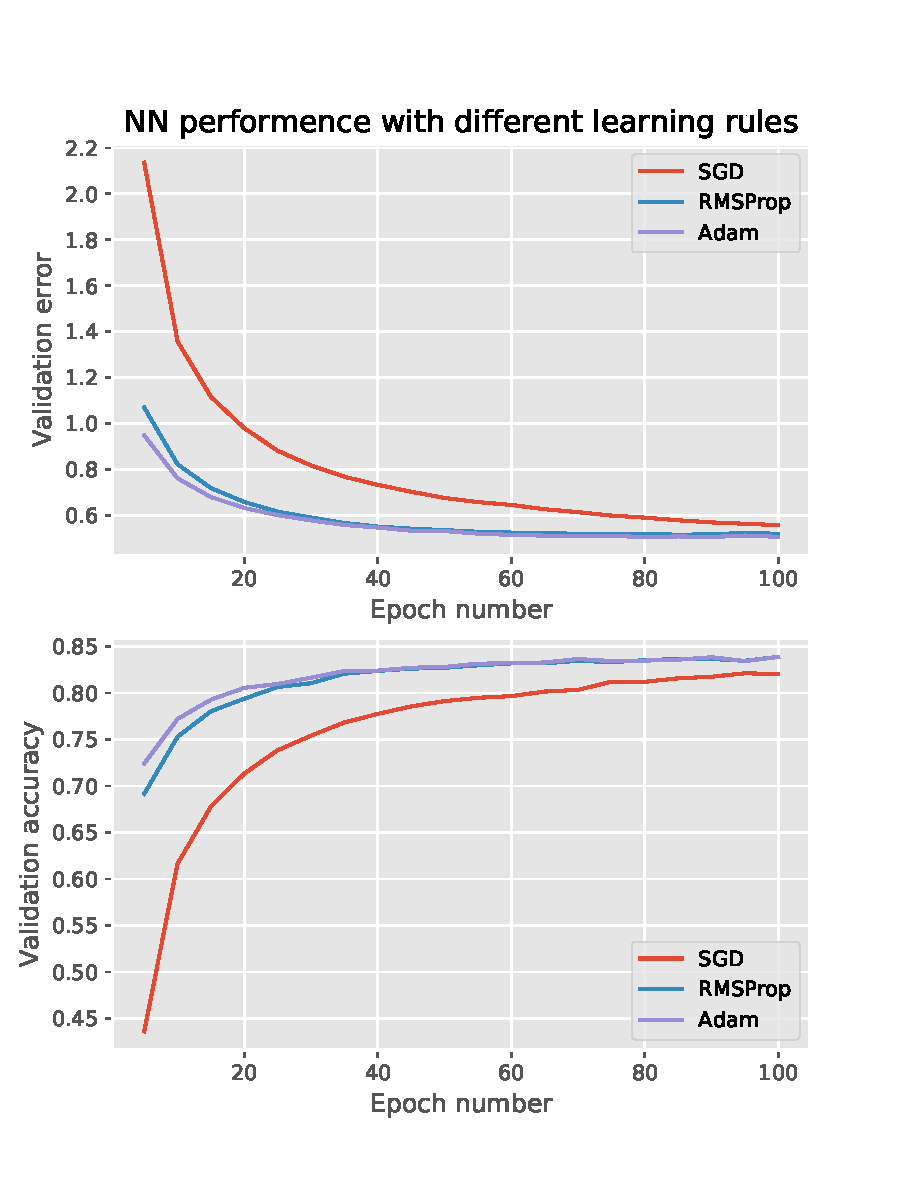
\includegraphics[width=\columnwidth]{ex2_comparison.pdf}}
\caption{Validation error over 200 training epochs}
\label{fig:ex2_compraison}
\end{center}
\end{figure} 

\section{Cosine annealing learning rate scheduler}
A variable learning rate has the potential to significantly to improve the performance of our learning algorithm if applied correctly. The inherit difficulty of this is that it adds more hyperparameter, thus increasing the complexity and human involvement \citep{loshchilov2018fixing}.

In this section we will implement a cosine annealing learning rate scheduler with warm restarts based on the paper by \citeauthor{loshchilov2018fixing}. This has been shown to improve anytime performance by quickly cooling down the learning rate according to a cosine schedule and periodically increasing it.

\subsection{Implementation}
Based on the above mentioned paper, cosine annealing has been implemented as a learning rate scheduler by introducing a learning rate multiplier $\eta_t$ which is updated on each epoch run with
$$\eta_t = \eta_{min} + 0.5(\eta_{max} - \eta_{min})(1 + \cos{\dfrac{\pi T_{cur}}{T_i})}$$
where $n_{min}$ and $n_{max}$ are ranges for the multiplier and $T_{cur}$ accounts for how many epochs have been performed since the last restart. $T_i$ is the period after which a restart should be performed. A restart occurs when $T_{cur} = T_i$ and at each restart $T_i$ is multiplied by a factor $T_{mult}$ and $T_i = 0$.
\\
In addition to the above, I have also implemented a version of cosine annealing which is similar to the one above but also resets the momentum on each warm restart. This will be referred to as \texttt{CosineAnnealingWithWarmRestartsPlus}.
\\
It was discovered during this part of the coursework was that the skeleton code provided did not exactly reflect the paper \citep{loshchilov2018fixing} which aims is to decouple the learning rate $\alpha$ and it's multiplier $\eta_t$ resulting in no correlation between the 2 parameters. The main strength of this is that you can independently tune $\alpha$ and $\eta_t$. However, this is not reflected in the skeleton code provided for the coursework as it explicitly states \texttt{min\_learning\_rate} and \texttt{max\_learning\_rate} as parameters of the cosine annealing scheduler. This infers that $\alpha$ and $\eta_t$ have been combined into one.

\subsection{Results}
Due to the above mentioned limitation, it proved to be difficult to experiment and choose appropriate parameters. Instead, the parameters were chosen using the method described in \citep{SGDR}, $\eta_{max} = \alpha$ where $\alpha$ is a learning rate that worked well before cosine annealing was applied and $\eta_{min}$ was chosen to be 2 magnitudes less based on the pseudo algorithmic scale mentioned in Section 2. That translates to $\eta_{max} = 0.005$ and $\eta_{min} = 0.0005$ for SGD and $\eta_{max} = 0.0001$ and $\eta_{min} = 0.00001$ for Adam. This is intuitive as in the worst case $\alpha$ will always be reset to it's maximum value (the value that worked best in previous experiments) and in the best case, a lower $\alpha$ will fit the dataset better. However, this might also result in overfitting.
\\
Multiple experiments were run with 3 different learning rate policies:
\begin{enumerate}
    \itemsep0em 
    \item Constant learning rate
    \item Cosine annealing with no warm restarts
    \item Cosine annealing with warm restarts with parameters $T_i = 25$, $T_{mult} = 3$ and $\alpha_{mult} = 0.9$ 
\end{enumerate}
with a neural network architecture similar to the one in the previous section but with varying learning rules between SGD and Adam.

From the results in Figure \ref{fig:ex3_sgd}, it can be seen that cosine annealing without restarts and constant $\alpha$ have very similar performance but cosine annealing with restarts is significantly slower to train. However, it seems that if the algorithm was given more training time, cosine annealing with restarts would have outperformed the other methods. \texttt{CosineAnnealingWithWarmRestartsPlus} does not seem to offer much of an improvement over the version it is based on.

\begin{figure}[tb]
\vskip 5mm
\begin{center}
\centerline{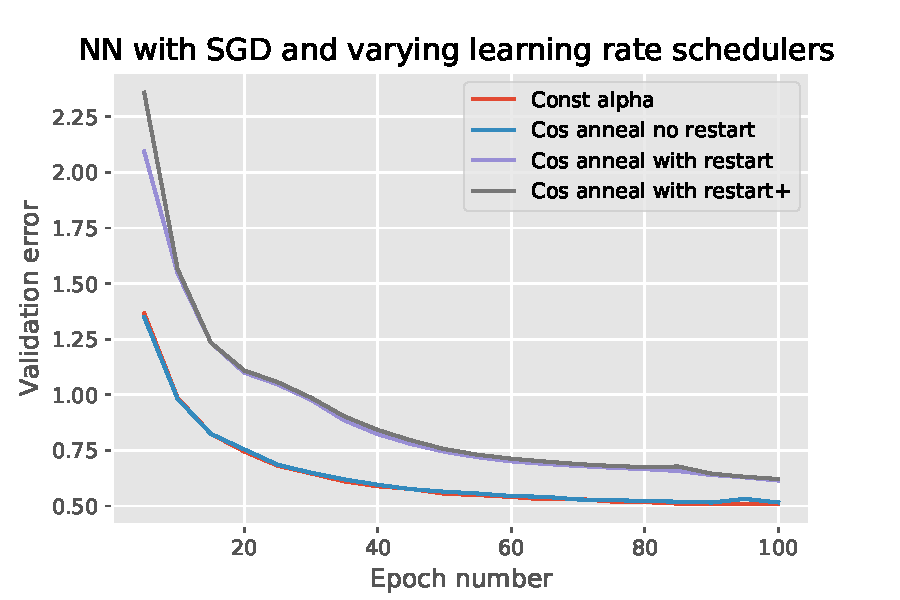
\includegraphics[width=\columnwidth]{ex3_sgd_comparison.pdf}}
\caption{Error with SGD optimisation and different learning rate policies}
\label{fig:ex3_sgd}
\end{center}
\vskip -5mm
\end{figure}

From the results in Figure \ref{fig:ex3_adam}, for Adam most of the results are analogous to SGD. Due to the faster rate of convergence of Adam, cosine annealing with restarts nearly outperforms the other techniques. It is also worth noting that the results are similar in the paper by \citeauthor{loshchilov2018fixing} where they even run for 2000 epochs. An interesting phenomenon is \texttt{CosineAnnealingWithWarmRestartsPlus} which has produced explainable results.

\begin{figure}[tb]
\vskip 5mm
\begin{center}
\centerline{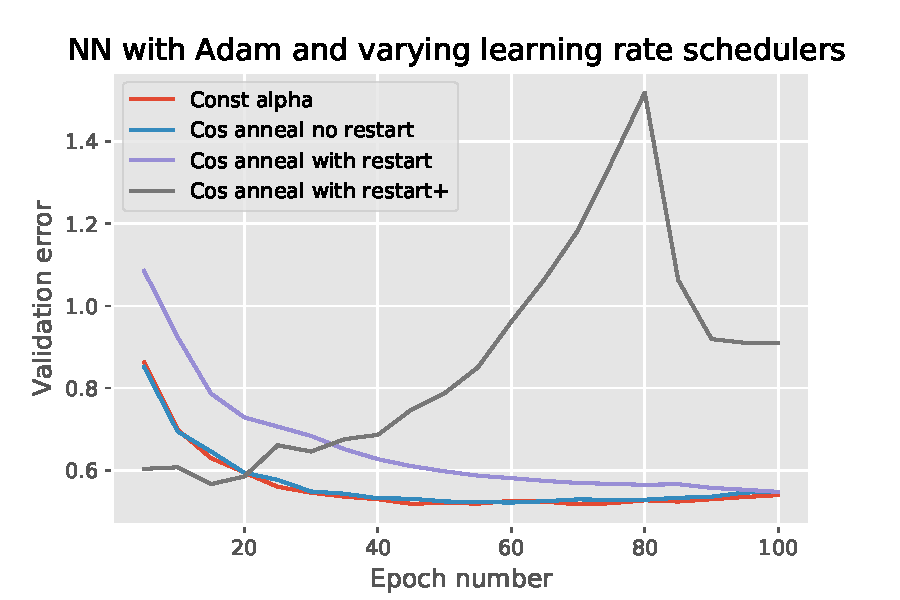
\includegraphics[width=\columnwidth]{ex3_adam_comparison.pdf}}
\caption{Error with Adam optimisation and different learning rate policies}
\label{fig:ex3_adam}
\end{center}
\vskip -5mm
\end{figure}

\section{Regularization and weight decay with Adam}

In the paper by \citeauthor{loshchilov2018fixing} it is described that one of the fundamental issues with Adam learning rules today is that they employ L2 regularisation instead of weight decay. When using the latter it changes the summed gradient of the regulariser and the loss function, whereas with weight decay only the gradients of the loss functions are changed (with the weight decay step separated from the
adaptive gradient mechanism). In this section we will explore both options, compare them and investigate how they affect the rest of the learning system.

\subsection{L2 Regularisation vs Weight decay}
First we must explore parameter options for both regularisation techniques in order to find the best factor. For that purpose the same Neural Network will be used as in the previous section. However, here we will consider only the Adam learning rule with $\alpha = 0.0001$. The weight decay/L2 regularisation factors that are explored are $[1^{-6}, 1^{-5}, 1^{-4}, 1^{-3}, 1^{-2}]$.
\\
For L2 regularisation it should be noted that $\alpha$ and the L2 factor are not decoupled and would indirectly affect each other. Although this effect is worth exploring with a technique like grid search, this would also require significant amount of time, thus it will not be explored here. This is not an issue for weight decay.
\\
For L2 regularisation it can be seen in Figure \ref{fig:ex4_l2} (in the Appendix) that there are only subtle differences between the choice of parameters but 0.001 is the clear winner resulting in 84,27\% accuracy rate.
\\
For weight decay, parameter choice is significantly more important as some choices even resulted in near 0 accuracy on validation data. However, choosing a parameter of value $1^{-5}$ resulted in the best performance with accuracy of 84,39\% on validation data. This can be observed in Figure \ref{fig:ex4_wd} (in the Appendix).

Now taking the best parameters for the above mentioned techniques and plotting them against a training session without any regularisation in Figure \ref{fig:ex4_lw_vs_wd}. It is clear to see the benefit of both of the newly introduced methods over learning a model with no regularisation. However, the difference between L2 regularisation and weight decay is subtle and can be attributed to not exploring enough values of weight decay factor. 


In conclusion the best accuracy achieved by Weight decay is 84,39\% . This confirms the results by \citeauthor{loshchilov2018fixing}. Therefore for the remainder of this section only weight decay with factor = $1^{-5}$ will be used.
\begin{figure}[tb]
\vskip 5mm
\begin{center}
\centerline{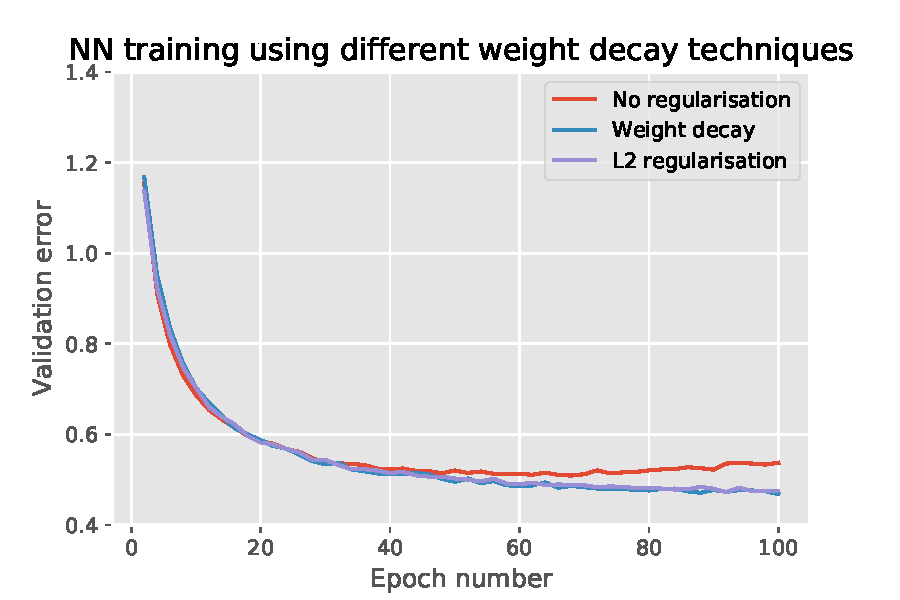
\includegraphics[width=\columnwidth]{ex4_l2_vs_wd.pdf}}
\caption{Error with different weight decay techniques}
\label{fig:ex4_lw_vs_wd}
\end{center}
\vskip -5mm
\end{figure}

\subsection{Effect on learning rate schedulers}
For this section we will assume that the learning rate scheduler is completely decoupled from the weight decay constant explored in the previous subsection. Furthermore the same neural network architecture will be used as in the previous subsection as well as the best parameters discovered for cosine annealing in Section 3. As seen in Figure \ref{fig:ex4_wd_cos_anneal}, warm restarts do not improve the performance of the algorithm, instead it results in overfitting as seen with the peaks of the error rate.

\begin{figure}[tb]
\vskip 5mm
\begin{center}
\centerline{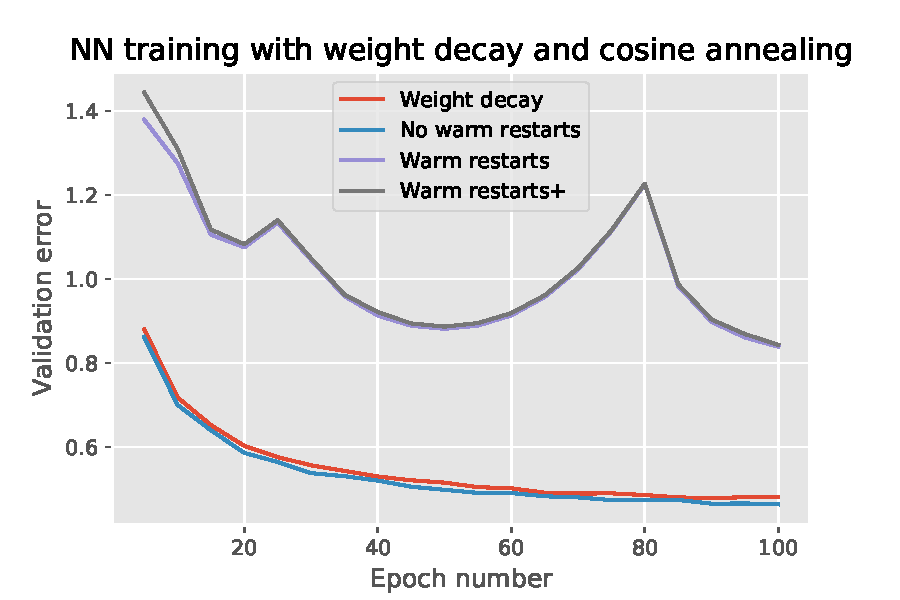
\includegraphics[width=\columnwidth]{ex4_wd_cos_anneal.pdf}}
\caption{Error with different weight decay techniques}
\label{fig:ex4_wd_cos_anneal}
\end{center}
\vskip -5mm
\end{figure}

\section{Conclusions}
\label{sec:concl}
All major algorithms and combinations of techniques are summarised in Figure \ref{fig:conclusion} for validation data and their real performance on test data is shown in Table \ref{tab:conclusions} where WD stands for weight decay and CA stands for cosine annealing with warm restarts.

\begin{table}[tb]
\begin{center}
\begin{small}
\begin{sc}
\begin{tabular}{lcccc}
\hline
\abovespace\belowspace
Method & Train acc & Valid acc & Test acc & Time (s) \\
\hline
\abovespace
SGD                     & 84,82 & 81,17 & 79,89 & 440 \\
RMSProp                 & 89,83 & 83,34 & 82,38 & 207 \\
Adam                    & 90,31 & 83,70 & 82,58 & 306 \\
SGD + CA                & 89,97 & 81,82 & 81,39 & 422 \\
Adam + WD               & 88,04 & 84,16 & 83,31 & 335 \\
Adam + WD + CA          & 76,03 & 75,59 & 74,49 & 342 \\
\hline
\end{tabular}
\end{sc}
\end{small}
\caption{Learning performance with varying learning rate.}
\label{tab:conclusions}
\end{center}
\end{table}

\begin{figure}[tb]
\begin{center}
\centerline{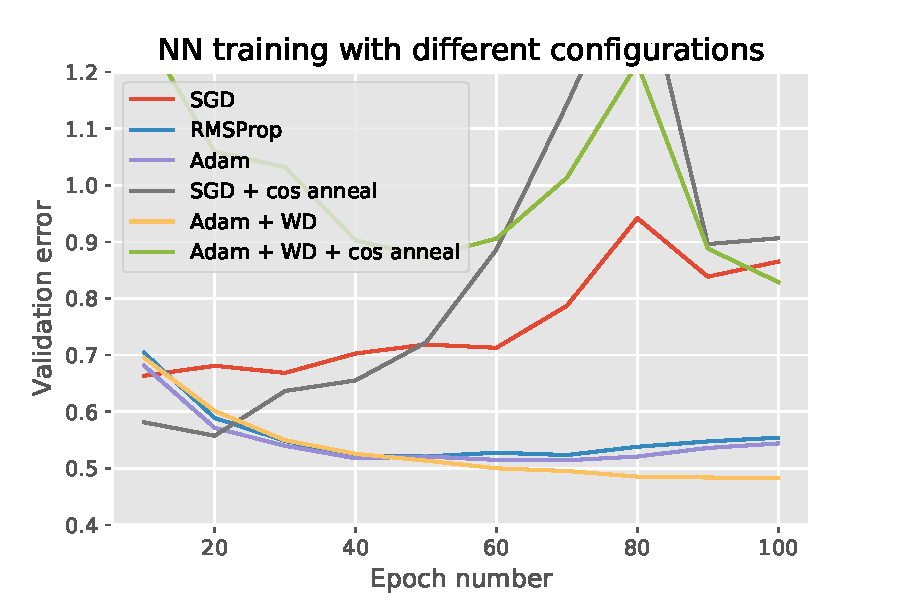
\includegraphics[width=\columnwidth]{conclusion.pdf}}
\caption{Validation error with different training techniques}
\label{fig:conclusion}
\end{center}
\end{figure}

It is clear to see that using Adam with weight decay is the most successful technique achieving 83,31\% accuracy on test data making it the best generalising method while also being the one with the lowest training time. This was achieved with hyperparameters $\alpha = 0.0001$, weight decay factor of $1^{-5}$, $ep = 100$, 3 hidden layers of 100 neurons each and a batch size of 100. These results confirms the findings by \citeauthor{overviewML} stating that Adam optimisation provides the most optimal performance on an image classification task. However, cosine annealing has not proven effective and adds more hyperparameter tuning complexity.

The findings presented in this section are interesting, however most experiments in this paper have been run for 100 epochs due to time limitations but we believe that in the future it is worth pursuing longer training runs.


% \section{Appendix}

\begin{appendices}

\begin{figure}[H]
\vskip 5mm
\begin{center}
\centerline{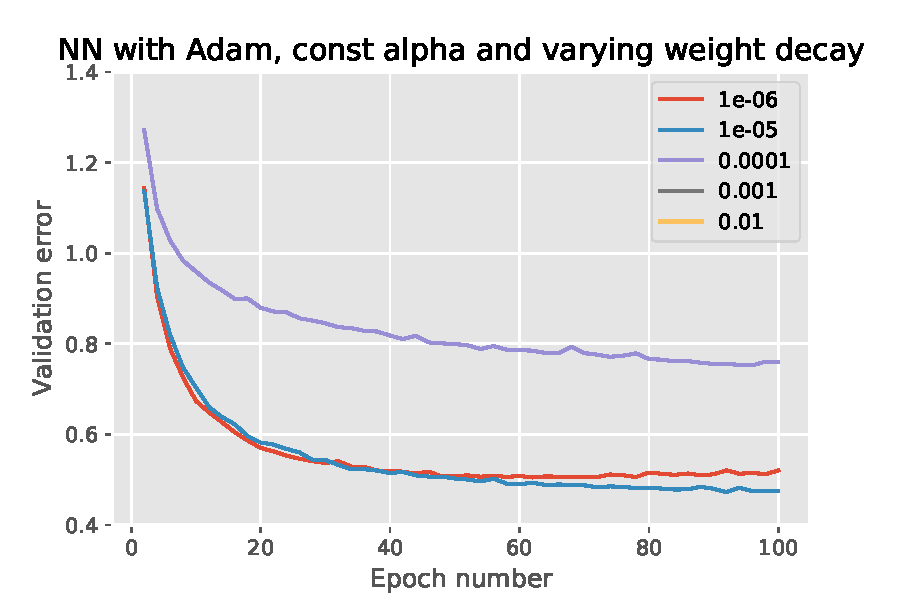
\includegraphics[width=\columnwidth]{ex4_wd_comparison.pdf}}
\caption{Error with Adam optimisation and varying weight decay factors}
\label{fig:ex4_wd}
\end{center}
\vskip -5mm
\end{figure}

\begin{figure}[H]
\vskip 5mm
\begin{center}
\centerline{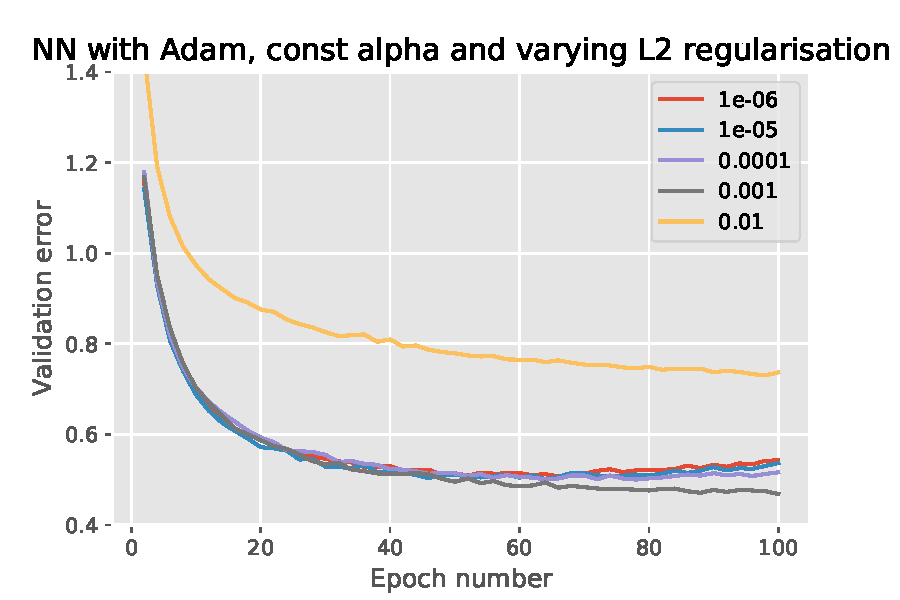
\includegraphics[width=\columnwidth]{ex4_l2_comparison.pdf}}
\caption{Error with Adam optimisation and varying L2 regularisation}
\label{fig:ex4_l2}
\end{center}
\vskip -5mm
\end{figure}

\end{appendices}

\vspace{70mm}

\bibliography{refs}


\end{document} 

